\documentclass[letterpaper]{article}

\usepackage[latin1]{inputenc}
\usepackage[brazil]{babel}
\usepackage{indentfirst}
\usepackage{fancyhdr}
\usepackage[noprefix]{nomencl}
\usepackage[letterpaper,
            ps2pdf,
            pdfborder={0 0 0},
            colorlinks={false},
            pdfpagemode={None},
            pdftitle={},
            pdfauthor={Victor de Abreu Iizuka et al},
            pdfsubject={RWA},
            pdfkeywords={RWA},
            pdfview={FitBH}]{hyperref}
\usepackage[T1]{fontenc}

\usepackage{graphicx}
\usepackage{setspace}
\usepackage{graphics}

\usepackage[algoruled,portugues,linesnumbered]{algorithm2e}
\usepackage{amsmath}
\usepackage{amsfonts}

%  ABACO -- Conjunto de macros para desenhar o 'abaco

%  Desenho original de Hans Liesenberg

%  Macros de Tomasz Kowaltowski

%  DCC -- IMECC -- UNICAMP

%  Mar,co de 1988  --  Vers~ao 1.0

% Ajustado para LaTeX da SUN -- Mar,co de 1991

% ---------------------------------------------------------

%  Chamada:   \ABACO{d1}{d2}{d3}{d4}{esc}
%             com:  di's -- os quatro d'igitos;
%	           esc  -- fator de escala

% ---------------------------------------------------------

%  DEFINI,C~OES AUXILIARES

% ---------------------------------------------------------


%  Forma o d'igito pequeno (0 ou 1)

\newcommand{\ABACODP}[1]{%
%
\thicklines
%    
\begin{picture}(8,0)
    \ifcase#1{   %  caso 0
       \put(0,0)    {\line(1,0){4}}
       \multiput(5,0)(2,0){2}{\oval(2,4)}}
    \or{         %  caso 1
       \put(2,0)    {\line(1,0){4}}
       \multiput(1,0)(6,0){2}{\oval(2,4)}}
    \fi
\end{picture}
    } % \ABACODP

% Forma o d'igito grande (0 a 4)

\newcommand{\ABACODG}[1]{%
%
\thicklines
%    
\begin{picture}(14,0)
    \ifcase#1{   % caso 0
       \multiput(1,0)(2,0){5}{\oval(2,4)}}
       \put(10,0)   {\line(1,0){4}}
    \or{         % caso 1
       \multiput(1,0)(2,0){4}{\oval(2,4)}}
       \put(8,0)   {\line(1,0){4}}
       \put(13,0)   {\oval(2,4)}
    \or{         % caso 2
       \multiput(1,0)(2,0){3}{\oval(2,4)}
       \put(6,0)   {\line(1,0){4}}
       \multiput(11,0)(2,0){2}{\oval(2,4)}}
    \or{         % caso 3
       \multiput(1,0)(2,0){2}{\oval(2,4)}
       \put(4,0)   {\line(1,0){4}}
       \multiput(9,0)(2,0){3}{\oval(2,4)}}
    \or{         % caso 4
       \put(1,0)  {\oval(2,4)}}
       \put(2,0)   {\line(1,0){4}}
       \multiput(7,0)(2,0){4}{\oval(2,4)}
    \fi
\end{picture}
    } % \ABACODG
       
% Forma um d'igito (0 a 9)

\newcommand{\ABACOD}[1]{%
%
    \ifnum#1>9
       \errmessage{#1: Argumento invalido para ABACO}
    \fi
    \ifnum#1<0
       \errmessage{#1: Argumento invalido para ABACO}
    \fi
%
\begin{picture}(24,0)
%    
    \ifnum#1<5
       \put(16,0) {\ABACODP{0}}
    \else   
       \put(16,0) {\ABACODP{1}}
    \fi
%    
    \ifnum#1<5
       \put(0,0)  {\ABACODG{#1}}
    \else
       \ifcase#1\or \or \or \or
          \or  \put(0,0)  {\ABACODG{0}}
          \or  \put(0,0)  {\ABACODG{1}}
          \or  \put(0,0)  {\ABACODG{2}}
          \or  \put(0,0)  {\ABACODG{3}}
          \or  \put(0,0)  {\ABACODG{4}}
       \fi
    \fi   
\end{picture}
    } % \ABACOD
    
% -------------------------------------------------

%  DEFINI,C~AO PRINCIPAL
    
\newcommand{\ABACO}[5]{%
    \setlength{\unitlength}{#5mm}
%
    \thinlines
%   
\begin{picture}(28,25)
%   
% moldura
%
% externa
%
        \put(0,0)            {\line(0,1){25}}
        \put(0,0)            {\line(1,0){28}}
        \put(28,0)           {\line(0,1){25}}
        \put(0,25)           {\line(1,0){28}}
% interna
        \put(2,2)            {\line(0,1){21}}
	\put(26,2)           {\line(0,1){21}}
	\put(16,2)           {\line(0,1){21}}
	\put(18,2)           {\line(0,1){21}}
	\put(2,2)            {\line(1,0){14}}
	\put(16,2)           {\line(1,-1){1}}
	\put(17,1)           {\line(1,1){1}}
	\put(18,2)           {\line(1,0){8}}
	\put(2,23)           {\line(1,0){14}}
	\put(16,23)          {\line(1,1){1}}
	\put(17,24)          {\line(1,-1){1}}
	\put(18,23)          {\line(1,0){8}}
	\put(0,0)            {\line(1,1){2}}
	\put(0,25)           {\line(1,-1){2}}
	\put(28,0)           {\line(-1,1){2}}
	\put(28,25)          {\line(-1,-1){2}}
%
%   
% d'igitos
%
%   
       \put(2,20)  {\ABACOD{#1}}
       \put(2,15)  {\ABACOD{#2}}
       \put(2,10)  {\ABACOD{#3}}
       \put(2,5)   {\ABACOD{#4}}
%      
\end{picture}
    } % \ABACO
    


\pagestyle{fancy}
\addtolength{\headheight}{2pt}
\fancyhead{}
\fancyhead[L]{\large{\textsf{Victor de A. I.}}}
\fancyhead[R]{\textsl{\leftmark}}
\fancyfoot{}
\fancyfoot[R]{\small{\textsl{pg. \thepage{} de \pageref{fimdoc}}}}
\fancyfoot[C]{\small{\textsf{Problema RWA}}}
\fancyfoot[L]{\small{\textsl{\today}}}
\renewcommand{\footrulewidth}{0.4pt}

\newcommand{\aspas}[1]{``#1''}
\newcommand{\estr}[1]{\textsl{\foreignlanguage{american}{#1}}}
\newcommand{\thead}[1]{\textbf{#1}}
\newcommand{\sigla}[1]{\texttt{#1}}
\newcommand{\converter}[2]{\small\textsl{#1 $\pm{}$ #2}\normalsize}
\newcommand{\rwa}{problema de roteamento e aloca��o de comprimentos de onda}
\newcommand{\wa}{problema de aloca��o de comprimentos de onda}
\hyphenation{e-xa-ta}

\title{
  \parbox{1in}{\ABACO{2}{0}{0}{9}{0.8}}
  \parbox{3in}{
    \normalsize{
      Universidade Estadual de Campinas - UNICAMP \\
      Instituto de Computa��o - IC 
    }
  }
  \vspace{3cm}\\
  \hspace{3cm}\\ \hspace{3cm}\\
  \Large{
    Algoritmo de roteamento para o problema RWA Parametrizado
  }\hfill \\
  \vspace{2cm}
  % \vspace*{2ex}
}

\author{
  \vspace{0.5cm}
  Victor de Abreu Iizuka  --- RA:046874 \\
  Prof. Edmundo Roberto Mauro Madeira \\
  Prof. Nelson Luis Saldanha da Fonseca \\
  \vspace{1cm}
}

%\date{}

\begin{document}

\maketitle{}
\newpage{}

\tableofcontents{}
\listoffigures{}
\listofalgorithms{}

\thispagestyle{empty}
\newpage{}

\section{Introdu��o}
\label{sec:intro}

O problema de roteamento e aloca��o de comprimentos de onda (RWA) em redes
com multiplexa��o por comprimento de ondas (WDM) procura definir as rotas
e os comprimentos de onda a serem alocados para caminhos �pticos. Procuramos
minimizar o n�mero de comprimentos de ondas utilizados para atender uma 
determinada demanda para diminuir o n�mero de \textit{transponder}\footnote{
  Equipamento que efetua a convers�o opto-eletro-�ptica.} necess�rios
nos comutadores de borda, diminu�ndo o custo da rede. O \rwa{} �, comumente,
resolvido em duas etapas, uma para definir o roteamento da demanda e a 
outra para alocar os comprimentos de ondas para estabelecer os caminhos 
que atendem as demandas de transporte \cite{RamMuk2002}.

\section{Modelo}
\label{subsec:model}

Uma rede �ptica pode ser modelada como um grafo $R = (G, V)$ no qual cada
aresta corresponde a um enlace de fibra. Uma requisi��o $r = [u, v]$ para
o estabelecimento de uma nova conex�o entre os n�s $u$ e $v$ � satisfeita
se:

\begin{itemize}
\item{um caminho $p_{r}$ com enlaces pertencentes a $R$ de $u$ a $v$ � 
  alocado para $r$.}
\item{um comprimento de onda que carrega a informa��o atrav�s dos enlaces
  de $p_{r}$ � alocado para $p_{r}$.}
\end{itemize}

Na solu��o do problema de RWA, se dois caminhos $p_{r}$ e $p_{r'}$, alocados
para as requisi��es $r$ e $r'$, possu�rem pelo menos um enlace em comum,
diferentes comprimentos de onda deveram ser alocadas para cada um dos 
caminhos. A formula��o cl�ssica em redes �pticas transparentes\footnote{
  Redes que n�o efetuam convers�o �ptico-eletr�nica.} assume que n�o h�
convers�o de comprimentos de onda.

\subsection{Grafo auxiliar}
\label{subsubsec:gaux}

Uma forma de modelar o problema de \wa{} em redes transparentes � criar um 
grafo auxiliar n�o direcionado no qual cada v�rtice corresponde a um 
caminho �ptico na rede. Dois v�rtices s�o ligados por uma aresta se existir
pelo menos um enlace �ptico compartilhado entre eles. Ap�s a gera��o do 
grafo auxiliar, calcula-se uma colora��o m�nima de v�rtices de forma que 
dois v�rtices adjacentes sempre recebam cores diferentes. No final temos
que cada caminho �ptico possui uma cor, que � mapeada nos respectivos 
comprimentos de onda.

\begin{figure}
  \begin{center}
      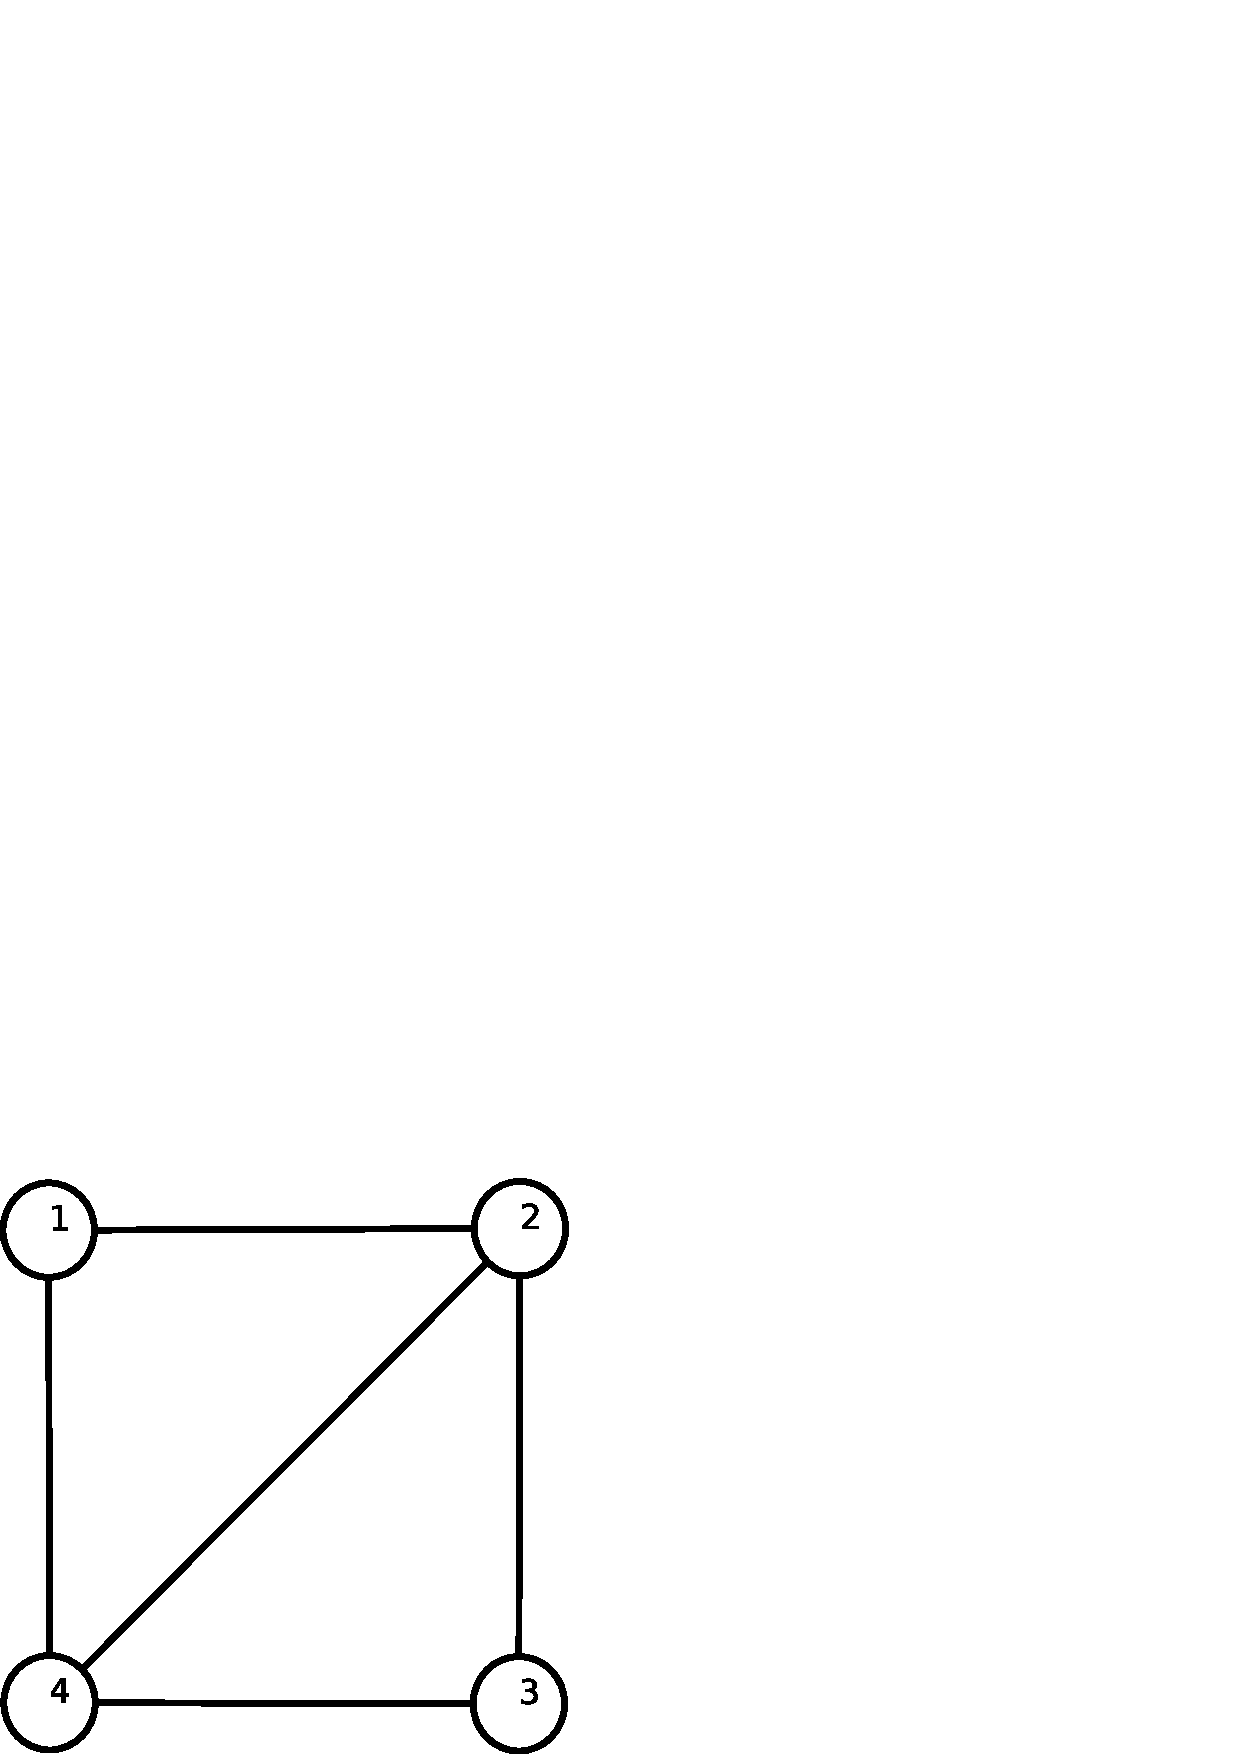
\includegraphics[bb=0 0 273 277, width=4cm]{fig/physical_topology-simple.pdf}
      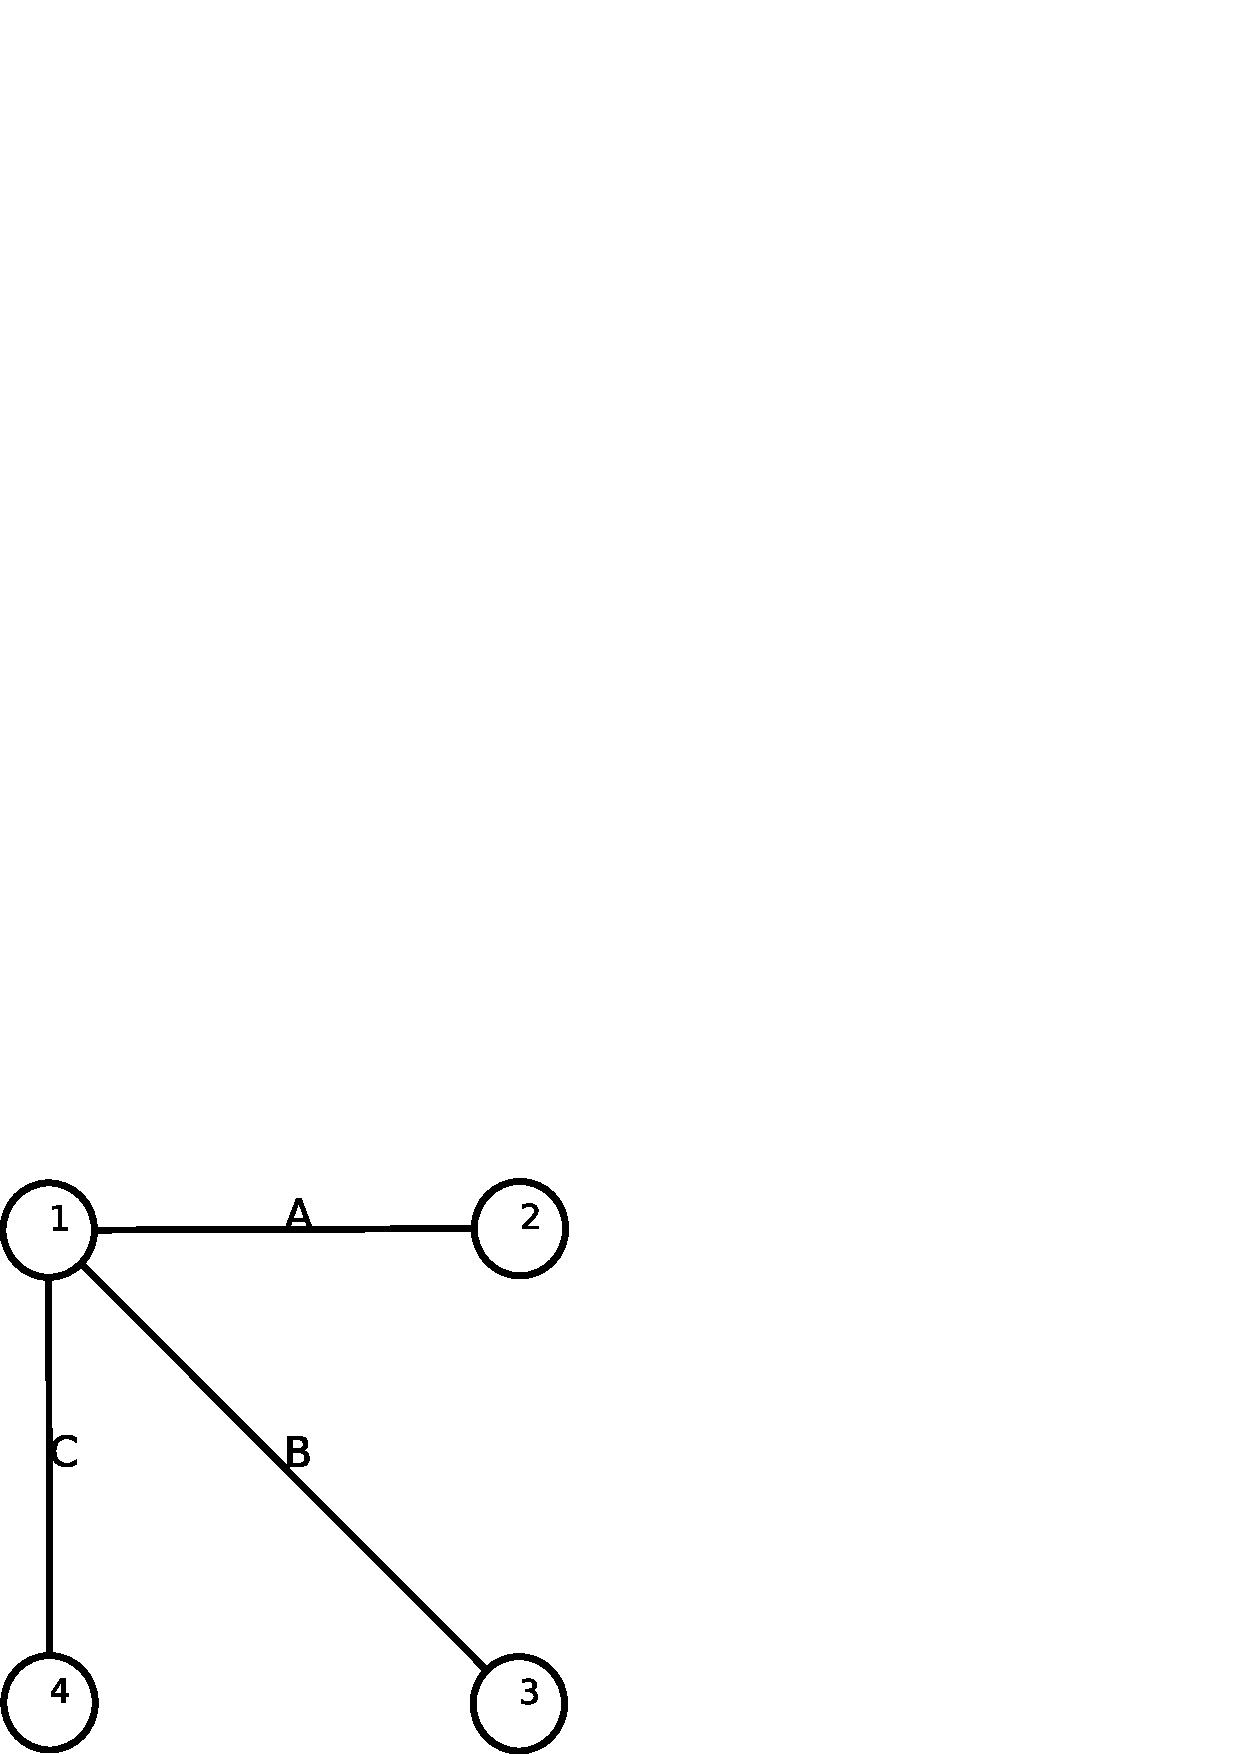
\includegraphics[bb=0 0 273 277, width=4cm]{fig/virtual_topology-simple.pdf}
  \end{center}

\caption{Topologia da rede �ptica e a sua topologia virtual.}
\end{figure}

\begin{figure}
  \begin{center}
    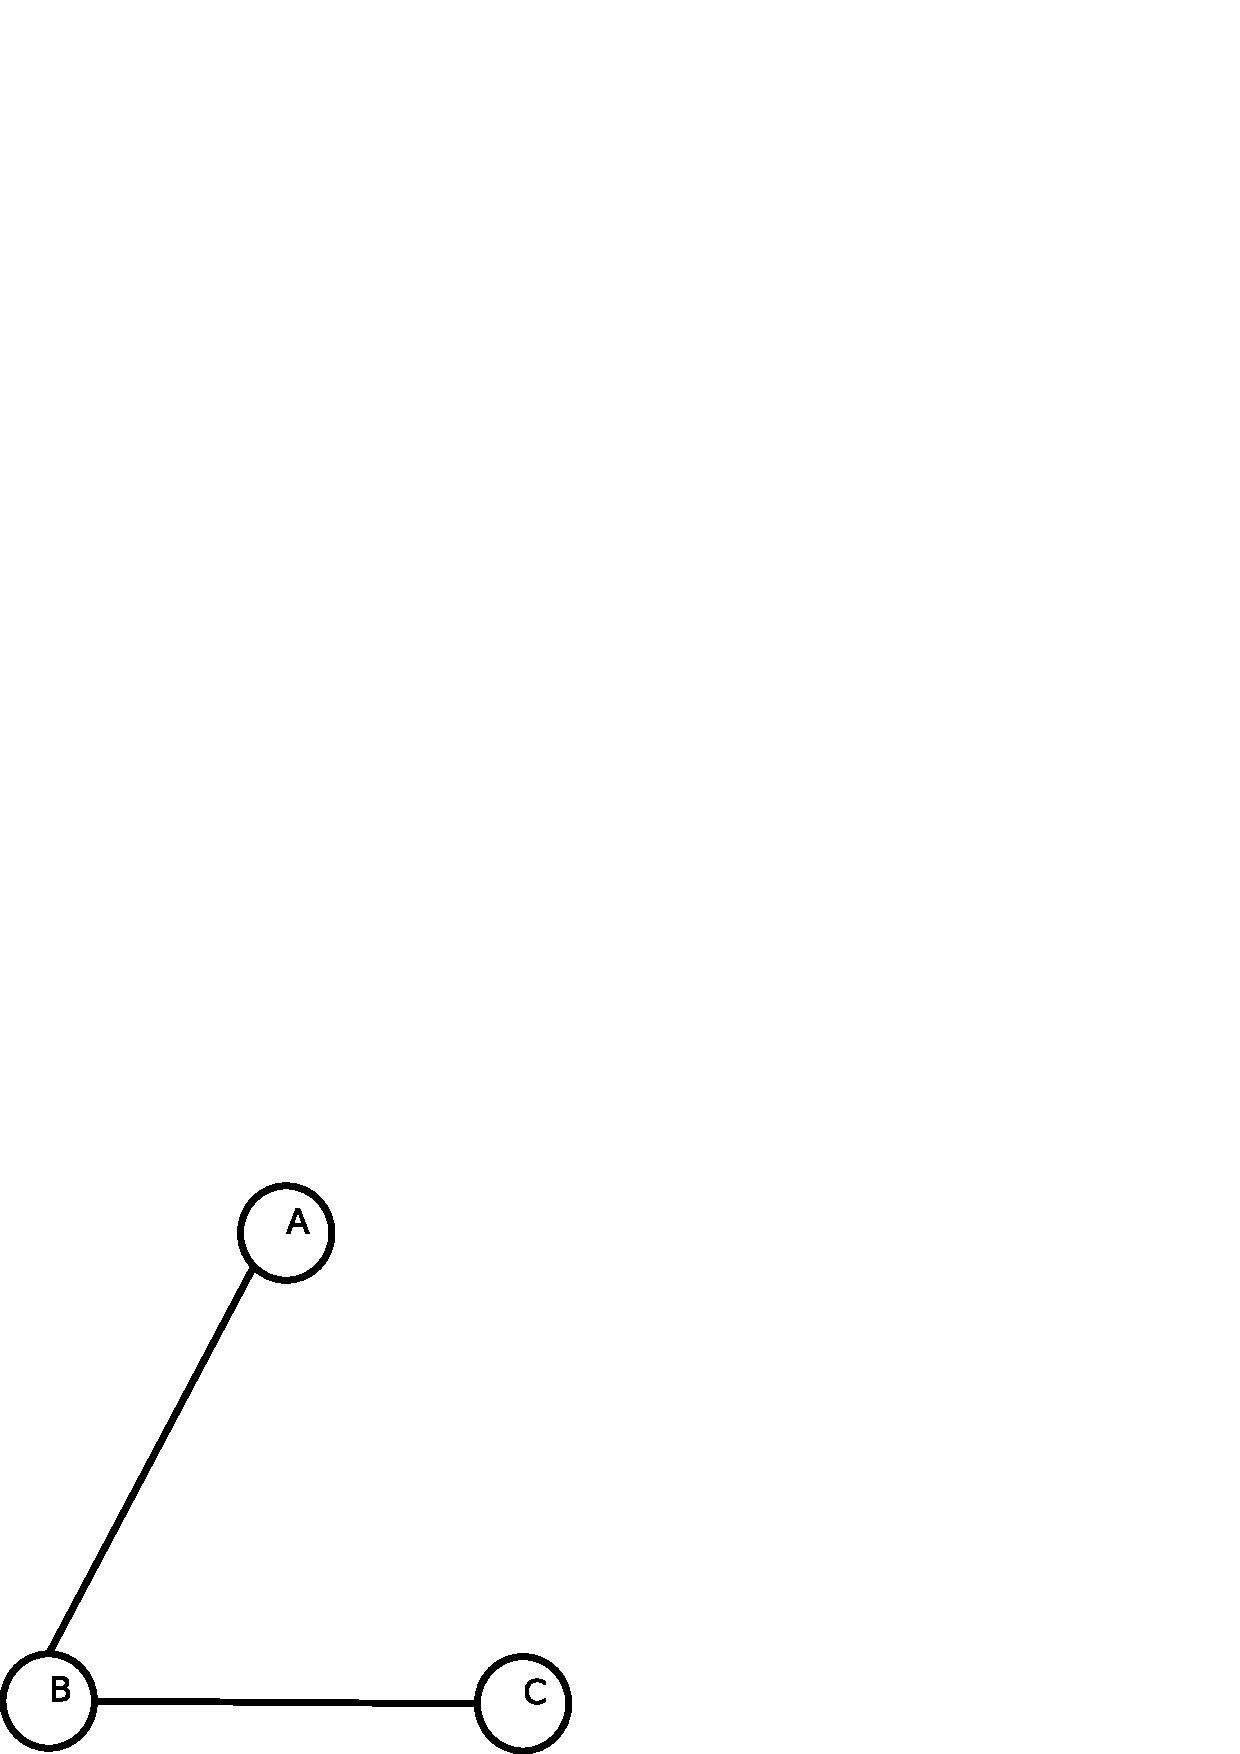
\includegraphics[bb=0 0 275 275, width=4cm]{fig/auxiliar_graph-simple.pdf}
    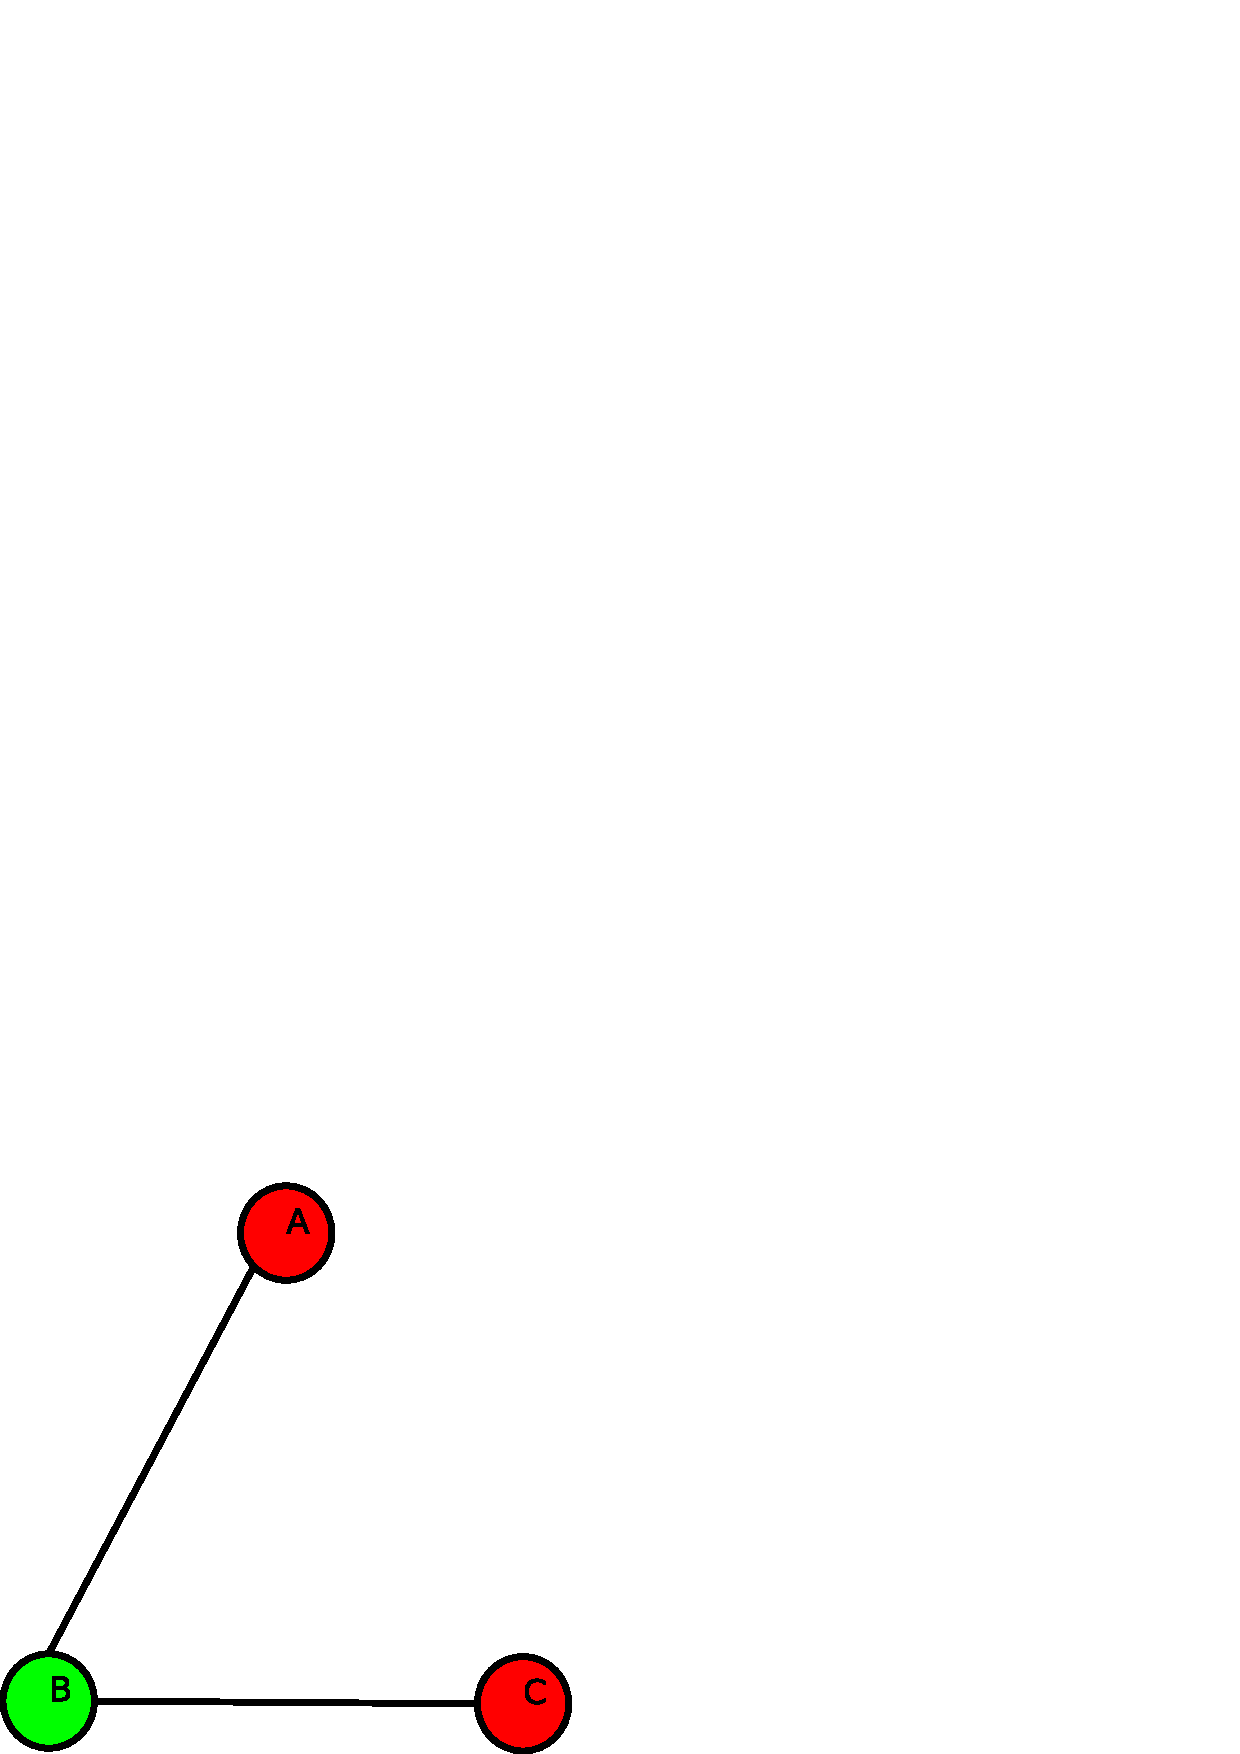
\includegraphics[bb=0 0 275 275, width=4cm]{fig/auxiliar_graph_color-simple.pdf}
  \end{center}

\caption{Grafo auxiliar e a sua colora��o m�nima de v�rtices.}
\end{figure}

\begin{figure}
  \begin{center}
    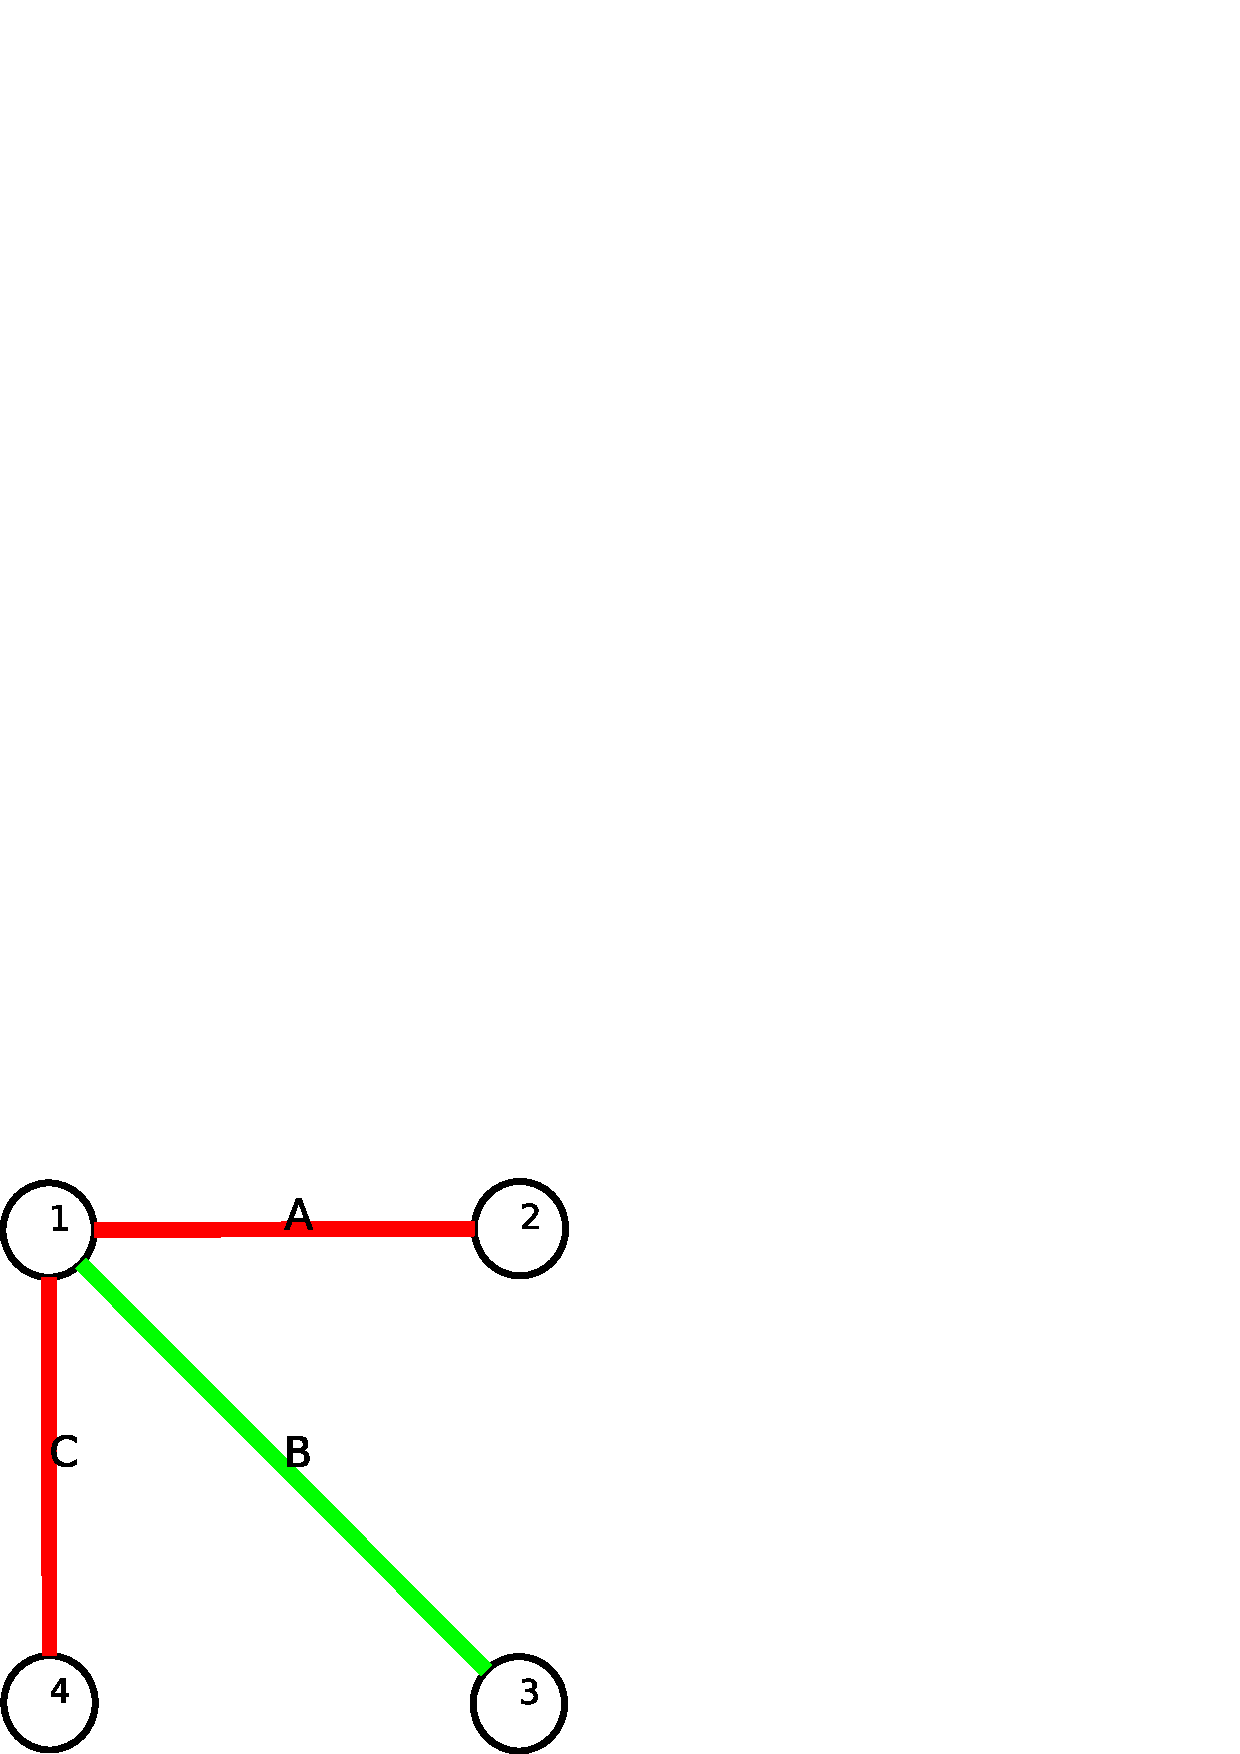
\includegraphics[bb=0 0 273 277, width=4cm]{fig/virtual_topology_color-simple.pdf}
    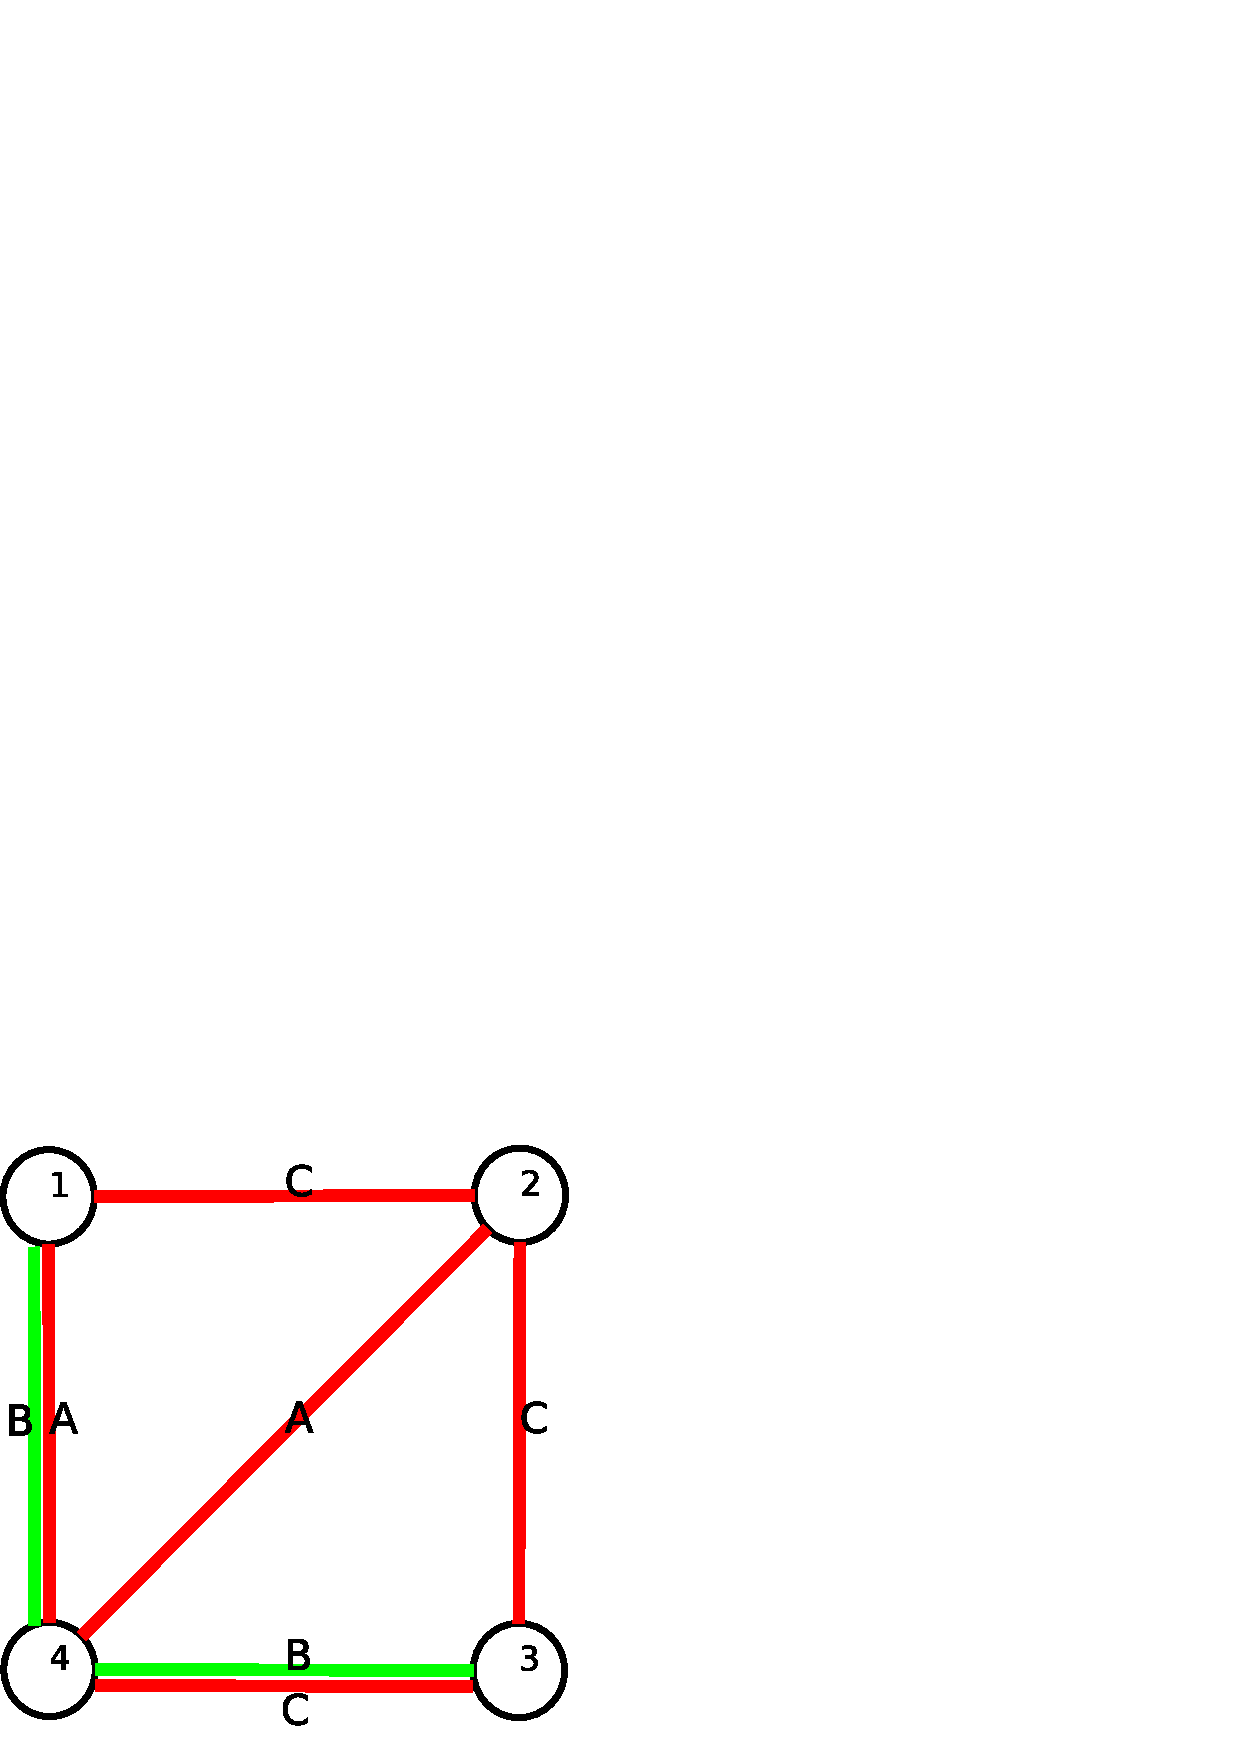
\includegraphics[bb=0 0 273 293, width=4cm]{fig/wavelength_assignment-simple.pdf}
  \end{center}

\caption{Colora��o sobre a Topologia Virtual e a aloca��o de comprimento de onda correspondente a colora��o obtida.}
\end{figure}

Esta abordagem de colora��o de v�rtices sempre foi usada no desenvolvimento
de novas solu��es para o \wa{} em redes �pticas. Este problema pertence a
classe dos problemas NP-dif�cil. Na literatura heur�sticas s�o usadas para 
a obten��o de solu��es r�pidas.

\section{Teoria da Complexidade Parametrizada}
\label{sec:tcpar}

O artigo \cite{DrumFon} introduz um algoritmo para a obten��o de uma 
solu��o exata do \wa{} usando a Teoria da Complexidade Parametrizada \cite{Downey}.
A Teoria da Complexidade Parametrizada foi recentemente proposta e introduz
a no��o de tratabilidade por par�metro-fixo (FPT) na remodelagem de problemas
dif�ceis, removendo a exponenciabilidade da complexidade do problema original.

O problema de colora��o �tima para um grafo da classe $F - ke$\footnote{
  Classe de grafos que pode ser obtida a partir de $F$ removendo no m�ximo 
  $k$ arestas} � FPT se o problema de colora��o para um grafo da classe $F$
pode ser resolvido em tempo polinomial e o problema para encontrar um 
Modulador\footnote{Conjunto de $k$ arestas que, quando adicionados, 
transformam um grafo $G$ em grafo da classe $F$.} para o grafo da classe 
$F - ke$ for FPT.

O algoritmo apresentado utiliza o fato que a o problema da colora��o 
m�nima de v�rtices em grafos da classe cordal\footnote{Grafos que n�o 
  possuem ciclos induzidos com mais de 3 v�rtices.} pode ser resolvido 
em complexidade de tempo linear no n�mero de v�rtices do grafo. Com isso,
o algoritmo possui uma complexidade de tempo de 
$O\left( \frac{4^k}{(k+1)^{\frac{3}{2}}}(m+n)\right)$, que � uma fun��o 
linear no tamanho da entrada ($n$ e $m$), e uma fun��o exponencial do 
par�metro $k$\footnote{Tamanho do Modulador}.

\section{Algoritmo}
\label{sec:alg}

\subsection{Obtendo o Grafo Cordal}
\label{subsec:gcordal}

Para obter um grafo auxiliar quasi-cordal � necess�rio evitar uma rela��o 
de interfer�ncia que forme um ciclo fechado.

Usaremos os seguintes teoremas para garantir que o grafo auxiliar seja
cordal.

\textbf{Teorema 1:} Seja um grafo $G = (V, E)$ da classe cordal. 
Seja $x$ um novo v�rtice a ser inserido em $G$ ligando este a outros 
dois v�rtices $u$ e $v$ ($u \in G$ e $v \in G$). Seja $p$ o caminho m�nimo 
entre $u$ e $v$ em $G$ e seja $G' = (V', E')$, onde $V' = V \cup \{x\}$ e 
$E' = E \cup \{(x, u), (x, v)\}$. O �nico buraco, se houver um, �
$p' = (x, u) + p + (x, v)$.

\textbf{Prova:} Como $G$ � cordal, o �nico poss�vel buraco deve passar 
por $x$, usando as novas arestas $(x, u)$ e $(x, v)$.

Se realmente houver um buraco em $G'$ faremos uma 
triangula��o acrescentando arestas entre $x$ e todo v�rtice 
de $p' - \{u, v\}$.

\textbf{Teorema 2:} Ap�s a triangulariza��o de $G'$ temos que $G'$ � cordal.

\textbf{Prova:} Pelo Teorema anterior o �nico buraco poss�vel em $G'$ � 
$p' = (x, u) + p + (x, v)$.\\
Ap�s a triangula��o este buraco � desfeito. Para quaisquer 3 v�rtices
ou mais de $p'$ juntamente com $x$ que formem um ciclo, necess�riamente
h� uma corda pois $x$ � ligado a todos os v�rtices de $p'$.\\
Quaisquer 4 v�rtices de $G'$ menos $x$ n�o podem ter um buraco pois
$G$ � cordal.

Agora considere que iremos ligar o v�rtice $x$ a um outro v�rtice $t$ de 
$G$.

\textbf{Teorema 3:} Seja $G' = (V', E')$ o grafo obtido ap�s a triangula��o. 
Seja $G'' = (V', E'')$, onde $E'' = E' \cup \{(x, t), p''\}$ e 
$p'' = (t, \ldots, z)$ � o caminho m�nimo de t at� algum v�rtice
$z \in p' - \{x\}$. O �nico buraco, se houver um, em $G''$ �
$p''' = (x, z) + p'' + (x, t)$.

\textbf{Prova:} Como $G$ e $G'$ s�o cordais, o �nico poss�vel buraco deve usar
a nova aresta $(x, t)$.

Se realmente houver um buraco em $G''$ faremos uma triangula��o 
acrescentando arestas entre $x$ e todo v�rtice de $p''' - \{z, t\}$.

\textbf{Teorema 4:} Ap�s a triangulariza��o de $G''$ temos que $G''$ � cordal.

\textbf{Prova:} Similar ao Teorema 2.

\subsection{Encontrando a Rota M�nima}
\label{subsec:rota}

A cada demanda obtemos o grafo auxiliar $G$ e obtemos o conjunto de arestas
usadas na triangula��o de $G$, denominado $T$ (modulador).
Calculamos a a rota m�nima de $s$ at� $t$ com par�metro $\alpha$
e $T$ para calcular as penaliza��es.

Ent�o a rota m�nima pode ser definida como:

\begin{equation}
  \min_{r}\big( \sum_{e \in r} w(e) + |T| \cdot \alpha \big)
\end{equation}

Usaremos um algorimo Branch-and-Bound para encontrar a rota m�nima usando os
par�metros $\alpha$ e $T$ para calcular as penaliza��es.

\begin{algorithm}[H]
  \caption{Rota M�nima $(s, t)$}
  \Entrada{V�rtice origem s e v�rtice destino t.}
  \Saida{Melhor rota.}
  \BlankLine{}
  $p \leftarrow s$
  \tcc*[l]{rota cont�m inicialmente s}
  $w \leftarrow 0$
  \tcc*[l]{custo inicialmente � 0}
  $Best \leftarrow \{ \infty, \emptyset \}$
  \tcc*[l]{melhor solu��o come�a com custo $\infty$ e caminho vazio}
  $Rota(s, t, w, p)$\;
  \Retorna{$Best$}\;
  \label{alg:rota_minima}
\end{algorithm}

\begin{algorithm}[H]
  \caption{Rota $(s, t, w, p)$}
  \Entrada{V�rtice origem s, v�rtice destino t, custo atual w e 
    rota atual p.}
  \Saida{Melhor rota.}
  \BlankLine{}
  \ParaCada{$u \in V(R)$ vizinho de $s$ tal que $u \notin p$}{
    \eSe{$(u == t)$ e $((w + w(s, t) + \alpha \cdot |T|) < Best)$}{
      $Best \leftarrow \{(w + w(s, t) + \alpha \cdot |T|), p + (s, t)\}$\;
    }{
      \Se{$lower(u,t) + w + w(s, u) < Best$}{
        $Rota(u, t, w + w(s, u), p + u)$\;
      }
    }
  }
  \label{alg:rota}
\end{algorithm}

%\input{sections/result}
\section{Conclus�o}
\label{sec:conc}

O \wa{} � um problema chave para o gerenciamento das redes WDM.
Este problema est� na classe NP-dif�cil, mas utilizando a Teoria da
Complexidade Parametrizada foi poss�vel obter um algoritmo exato que 
pode explorar caracter�sticas n�o trivi�is do \wa{}. A Teoria de Complexidade
Parametrizada define novos horizontes para a aplica��o na aloca��o de comprimentos
de ondas em redes transparentes\footnote{Para outros problemas tamb�m.}, abrindo
espa�o para muitos outros trabalhos que utilizam essa t�cnica.



\bibliographystyle{plain}
\bibliography{ra046874}

\label{fimdoc}
\end{document}
